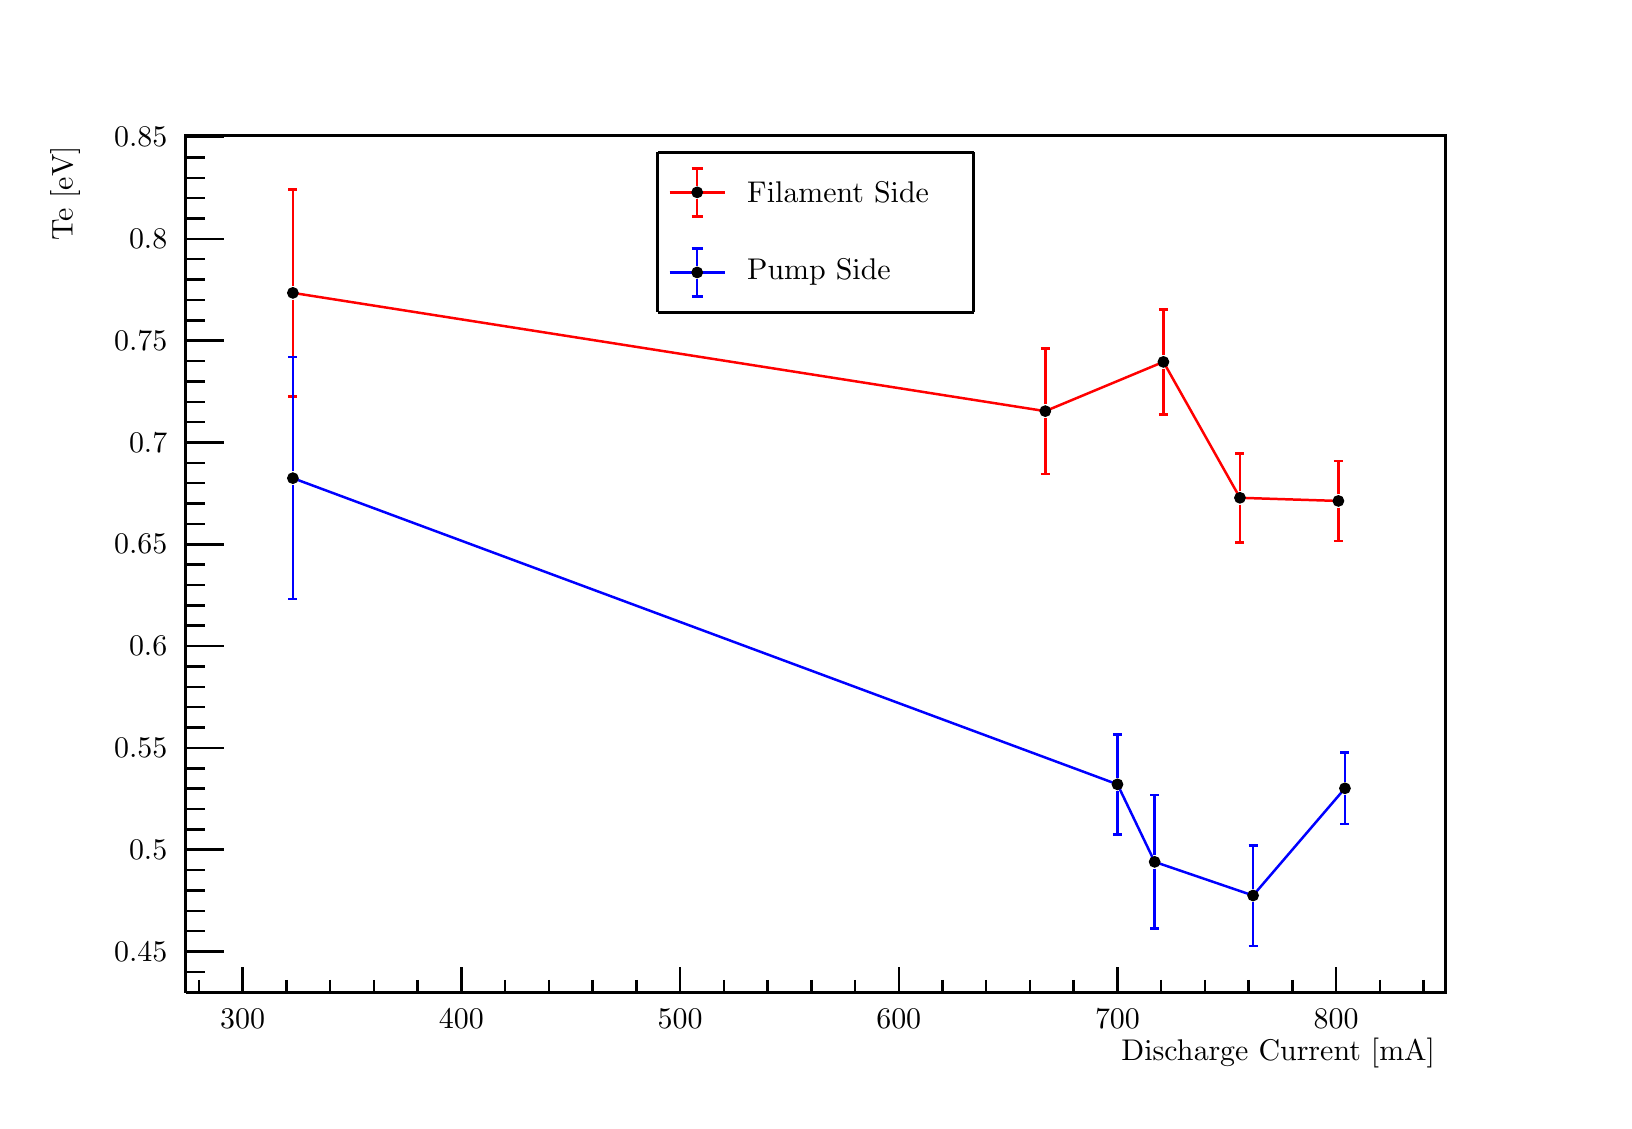
\begin{tikzpicture}
\pgfdeclareplotmark{cross} {
\pgfpathmoveto{\pgfpoint{-0.3\pgfplotmarksize}{\pgfplotmarksize}}
\pgfpathlineto{\pgfpoint{+0.3\pgfplotmarksize}{\pgfplotmarksize}}
\pgfpathlineto{\pgfpoint{+0.3\pgfplotmarksize}{0.3\pgfplotmarksize}}
\pgfpathlineto{\pgfpoint{+1\pgfplotmarksize}{0.3\pgfplotmarksize}}
\pgfpathlineto{\pgfpoint{+1\pgfplotmarksize}{-0.3\pgfplotmarksize}}
\pgfpathlineto{\pgfpoint{+0.3\pgfplotmarksize}{-0.3\pgfplotmarksize}}
\pgfpathlineto{\pgfpoint{+0.3\pgfplotmarksize}{-1.\pgfplotmarksize}}
\pgfpathlineto{\pgfpoint{-0.3\pgfplotmarksize}{-1.\pgfplotmarksize}}
\pgfpathlineto{\pgfpoint{-0.3\pgfplotmarksize}{-0.3\pgfplotmarksize}}
\pgfpathlineto{\pgfpoint{-1.\pgfplotmarksize}{-0.3\pgfplotmarksize}}
\pgfpathlineto{\pgfpoint{-1.\pgfplotmarksize}{0.3\pgfplotmarksize}}
\pgfpathlineto{\pgfpoint{-0.3\pgfplotmarksize}{0.3\pgfplotmarksize}}
\pgfpathclose
\pgfusepathqstroke
}
\pgfdeclareplotmark{cross*} {
\pgfpathmoveto{\pgfpoint{-0.3\pgfplotmarksize}{\pgfplotmarksize}}
\pgfpathlineto{\pgfpoint{+0.3\pgfplotmarksize}{\pgfplotmarksize}}
\pgfpathlineto{\pgfpoint{+0.3\pgfplotmarksize}{0.3\pgfplotmarksize}}
\pgfpathlineto{\pgfpoint{+1\pgfplotmarksize}{0.3\pgfplotmarksize}}
\pgfpathlineto{\pgfpoint{+1\pgfplotmarksize}{-0.3\pgfplotmarksize}}
\pgfpathlineto{\pgfpoint{+0.3\pgfplotmarksize}{-0.3\pgfplotmarksize}}
\pgfpathlineto{\pgfpoint{+0.3\pgfplotmarksize}{-1.\pgfplotmarksize}}
\pgfpathlineto{\pgfpoint{-0.3\pgfplotmarksize}{-1.\pgfplotmarksize}}
\pgfpathlineto{\pgfpoint{-0.3\pgfplotmarksize}{-0.3\pgfplotmarksize}}
\pgfpathlineto{\pgfpoint{-1.\pgfplotmarksize}{-0.3\pgfplotmarksize}}
\pgfpathlineto{\pgfpoint{-1.\pgfplotmarksize}{0.3\pgfplotmarksize}}
\pgfpathlineto{\pgfpoint{-0.3\pgfplotmarksize}{0.3\pgfplotmarksize}}
\pgfpathclose
\pgfusepathqfillstroke
}
\pgfdeclareplotmark{newstar} {
\pgfpathmoveto{\pgfqpoint{0pt}{\pgfplotmarksize}}
\pgfpathlineto{\pgfqpointpolar{44}{0.5\pgfplotmarksize}}
\pgfpathlineto{\pgfqpointpolar{18}{\pgfplotmarksize}}
\pgfpathlineto{\pgfqpointpolar{-20}{0.5\pgfplotmarksize}}
\pgfpathlineto{\pgfqpointpolar{-54}{\pgfplotmarksize}}
\pgfpathlineto{\pgfqpointpolar{-90}{0.5\pgfplotmarksize}}
\pgfpathlineto{\pgfqpointpolar{234}{\pgfplotmarksize}}
\pgfpathlineto{\pgfqpointpolar{198}{0.5\pgfplotmarksize}}
\pgfpathlineto{\pgfqpointpolar{162}{\pgfplotmarksize}}
\pgfpathlineto{\pgfqpointpolar{134}{0.5\pgfplotmarksize}}
\pgfpathclose
\pgfusepathqstroke
}
\pgfdeclareplotmark{newstar*} {
\pgfpathmoveto{\pgfqpoint{0pt}{\pgfplotmarksize}}
\pgfpathlineto{\pgfqpointpolar{44}{0.5\pgfplotmarksize}}
\pgfpathlineto{\pgfqpointpolar{18}{\pgfplotmarksize}}
\pgfpathlineto{\pgfqpointpolar{-20}{0.5\pgfplotmarksize}}
\pgfpathlineto{\pgfqpointpolar{-54}{\pgfplotmarksize}}
\pgfpathlineto{\pgfqpointpolar{-90}{0.5\pgfplotmarksize}}
\pgfpathlineto{\pgfqpointpolar{234}{\pgfplotmarksize}}
\pgfpathlineto{\pgfqpointpolar{198}{0.5\pgfplotmarksize}}
\pgfpathlineto{\pgfqpointpolar{162}{\pgfplotmarksize}}
\pgfpathlineto{\pgfqpointpolar{134}{0.5\pgfplotmarksize}}
\pgfpathclose
\pgfusepathqfillstroke
}
\definecolor{c}{rgb}{1,1,1};
\draw [color=c, fill=c] (0,0) rectangle (20,13.6103);
\draw [color=c, fill=c] (2,1.36103) rectangle (18,12.2493);
\definecolor{c}{rgb}{0,0,0};
\draw [c,line width=0.9] (2,1.36103) -- (2,12.2493) -- (18,12.2493) -- (18,1.36103) -- (2,1.36103);
\definecolor{c}{rgb}{1,1,1};
\draw [color=c, fill=c] (2,1.36103) rectangle (18,12.2493);
\definecolor{c}{rgb}{0,0,0};
\draw [c,line width=0.9] (2,1.36103) -- (2,12.2493) -- (18,12.2493) -- (18,1.36103) -- (2,1.36103);
\draw [c,line width=0.9] (2,1.36103) -- (18,1.36103);
\draw [c,line width=0.9] (2.72222,1.68768) -- (2.72222,1.36103);
\draw [c,line width=0.9] (3.27778,1.52436) -- (3.27778,1.36103);
\draw [c,line width=0.9] (3.83333,1.52436) -- (3.83333,1.36103);
\draw [c,line width=0.9] (4.38889,1.52436) -- (4.38889,1.36103);
\draw [c,line width=0.9] (4.94444,1.52436) -- (4.94444,1.36103);
\draw [c,line width=0.9] (5.5,1.68768) -- (5.5,1.36103);
\draw [c,line width=0.9] (6.05556,1.52436) -- (6.05556,1.36103);
\draw [c,line width=0.9] (6.61111,1.52436) -- (6.61111,1.36103);
\draw [c,line width=0.9] (7.16667,1.52436) -- (7.16667,1.36103);
\draw [c,line width=0.9] (7.72222,1.52436) -- (7.72222,1.36103);
\draw [c,line width=0.9] (8.27778,1.68768) -- (8.27778,1.36103);
\draw [c,line width=0.9] (8.83333,1.52436) -- (8.83333,1.36103);
\draw [c,line width=0.9] (9.38889,1.52436) -- (9.38889,1.36103);
\draw [c,line width=0.9] (9.94444,1.52436) -- (9.94444,1.36103);
\draw [c,line width=0.9] (10.5,1.52436) -- (10.5,1.36103);
\draw [c,line width=0.9] (11.0556,1.68768) -- (11.0556,1.36103);
\draw [c,line width=0.9] (11.6111,1.52436) -- (11.6111,1.36103);
\draw [c,line width=0.9] (12.1667,1.52436) -- (12.1667,1.36103);
\draw [c,line width=0.9] (12.7222,1.52436) -- (12.7222,1.36103);
\draw [c,line width=0.9] (13.2778,1.52436) -- (13.2778,1.36103);
\draw [c,line width=0.9] (13.8333,1.68768) -- (13.8333,1.36103);
\draw [c,line width=0.9] (14.3889,1.52436) -- (14.3889,1.36103);
\draw [c,line width=0.9] (14.9444,1.52436) -- (14.9444,1.36103);
\draw [c,line width=0.9] (15.5,1.52436) -- (15.5,1.36103);
\draw [c,line width=0.9] (16.0556,1.52436) -- (16.0556,1.36103);
\draw [c,line width=0.9] (16.6111,1.68768) -- (16.6111,1.36103);
\draw [c,line width=0.9] (2.72222,1.68768) -- (2.72222,1.36103);
\draw [c,line width=0.9] (2.16667,1.52436) -- (2.16667,1.36103);
\draw [c,line width=0.9] (16.6111,1.68768) -- (16.6111,1.36103);
\draw [c,line width=0.9] (17.1667,1.52436) -- (17.1667,1.36103);
\draw [c,line width=0.9] (17.7222,1.52436) -- (17.7222,1.36103);
\draw [anchor=base] (2.72222,0.911891) node[scale=1.08185, color=c, rotate=0]{300};
\draw [anchor=base] (5.5,0.911891) node[scale=1.08185, color=c, rotate=0]{400};
\draw [anchor=base] (8.27778,0.911891) node[scale=1.08185, color=c, rotate=0]{500};
\draw [anchor=base] (11.0556,0.911891) node[scale=1.08185, color=c, rotate=0]{600};
\draw [anchor=base] (13.8333,0.911891) node[scale=1.08185, color=c, rotate=0]{700};
\draw [anchor=base] (16.6111,0.911891) node[scale=1.08185, color=c, rotate=0]{800};
\draw [anchor= east] (18,0.598854) node[scale=1.08185, color=c, rotate=0]{Discharge Current [mA]};
\draw [c,line width=0.9] (2,1.36103) -- (2,12.2493);
\draw [c,line width=0.9] (2.48,1.88447) -- (2,1.88447);
\draw [c,line width=0.9] (2.24,2.14307) -- (2,2.14307);
\draw [c,line width=0.9] (2.24,2.40166) -- (2,2.40166);
\draw [c,line width=0.9] (2.24,2.66025) -- (2,2.66025);
\draw [c,line width=0.9] (2.24,2.91884) -- (2,2.91884);
\draw [c,line width=0.9] (2.48,3.17744) -- (2,3.17744);
\draw [c,line width=0.9] (2.24,3.43603) -- (2,3.43603);
\draw [c,line width=0.9] (2.24,3.69462) -- (2,3.69462);
\draw [c,line width=0.9] (2.24,3.95322) -- (2,3.95322);
\draw [c,line width=0.9] (2.24,4.21181) -- (2,4.21181);
\draw [c,line width=0.9] (2.48,4.4704) -- (2,4.4704);
\draw [c,line width=0.9] (2.24,4.72899) -- (2,4.72899);
\draw [c,line width=0.9] (2.24,4.98759) -- (2,4.98759);
\draw [c,line width=0.9] (2.24,5.24618) -- (2,5.24618);
\draw [c,line width=0.9] (2.24,5.50477) -- (2,5.50477);
\draw [c,line width=0.9] (2.48,5.76336) -- (2,5.76336);
\draw [c,line width=0.9] (2.24,6.02196) -- (2,6.02196);
\draw [c,line width=0.9] (2.24,6.28055) -- (2,6.28055);
\draw [c,line width=0.9] (2.24,6.53914) -- (2,6.53914);
\draw [c,line width=0.9] (2.24,6.79774) -- (2,6.79774);
\draw [c,line width=0.9] (2.48,7.05633) -- (2,7.05633);
\draw [c,line width=0.9] (2.24,7.31492) -- (2,7.31492);
\draw [c,line width=0.9] (2.24,7.57351) -- (2,7.57351);
\draw [c,line width=0.9] (2.24,7.83211) -- (2,7.83211);
\draw [c,line width=0.9] (2.24,8.0907) -- (2,8.0907);
\draw [c,line width=0.9] (2.48,8.34929) -- (2,8.34929);
\draw [c,line width=0.9] (2.24,8.60789) -- (2,8.60789);
\draw [c,line width=0.9] (2.24,8.86648) -- (2,8.86648);
\draw [c,line width=0.9] (2.24,9.12507) -- (2,9.12507);
\draw [c,line width=0.9] (2.24,9.38366) -- (2,9.38366);
\draw [c,line width=0.9] (2.48,9.64226) -- (2,9.64226);
\draw [c,line width=0.9] (2.24,9.90085) -- (2,9.90085);
\draw [c,line width=0.9] (2.24,10.1594) -- (2,10.1594);
\draw [c,line width=0.9] (2.24,10.418) -- (2,10.418);
\draw [c,line width=0.9] (2.24,10.6766) -- (2,10.6766);
\draw [c,line width=0.9] (2.48,10.9352) -- (2,10.9352);
\draw [c,line width=0.9] (2.24,11.1938) -- (2,11.1938);
\draw [c,line width=0.9] (2.24,11.4524) -- (2,11.4524);
\draw [c,line width=0.9] (2.24,11.711) -- (2,11.711);
\draw [c,line width=0.9] (2.24,11.9696) -- (2,11.9696);
\draw [c,line width=0.9] (2.48,12.2282) -- (2,12.2282);
\draw [c,line width=0.9] (2.48,1.88447) -- (2,1.88447);
\draw [c,line width=0.9] (2.24,1.62588) -- (2,1.62588);
\draw [c,line width=0.9] (2.24,1.36729) -- (2,1.36729);
\draw [c,line width=0.9] (2.48,12.2282) -- (2,12.2282);
\draw [anchor= east] (1.9,1.88447) node[scale=1.08185, color=c, rotate=0]{0.45};
\draw [anchor= east] (1.9,3.17744) node[scale=1.08185, color=c, rotate=0]{0.5};
\draw [anchor= east] (1.9,4.4704) node[scale=1.08185, color=c, rotate=0]{0.55};
\draw [anchor= east] (1.9,5.76336) node[scale=1.08185, color=c, rotate=0]{0.6};
\draw [anchor= east] (1.9,7.05633) node[scale=1.08185, color=c, rotate=0]{0.65};
\draw [anchor= east] (1.9,8.34929) node[scale=1.08185, color=c, rotate=0]{0.7};
\draw [anchor= east] (1.9,9.64226) node[scale=1.08185, color=c, rotate=0]{0.75};
\draw [anchor= east] (1.9,10.9352) node[scale=1.08185, color=c, rotate=0]{0.8};
\draw [anchor= east] (1.9,12.2282) node[scale=1.08185, color=c, rotate=0]{0.85};
\draw [anchor= east] (0.469055,12.2493) node[scale=1.08185, color=c, rotate=90]{Te [eV]};
\definecolor{c}{rgb}{1,0,0};
\draw [c,line width=0.9] (3.36111,10.2491) -- (12.9167,8.74724) -- (14.4167,9.3726) -- (15.3889,7.64662) -- (16.6389,7.60669);
\definecolor{c}{rgb}{0,0,0};
\foreach \P in {(3.36111,10.2491), (12.9167,8.74724), (14.4167,9.3726), (15.3889,7.64662), (16.6389,7.60669)}{\draw[mark options={color=c,fill=c},mark size=1.921922pt,mark=*] plot coordinates {\P};}
\definecolor{c}{rgb}{1,0,0};
\draw [c,line width=0.9] (3.36111,10.3351) -- (3.36111,11.5651);
\draw [c,line width=0.9] (3.3038,11.5651) -- (3.41842,11.5651);
\draw [c,line width=0.9] (3.36111,10.1632) -- (3.36111,8.93318);
\draw [c,line width=0.9] (3.3038,8.93318) -- (3.41842,8.93318);
\draw [c,line width=0.9] (12.9167,8.8332) -- (12.9167,9.54373);
\draw [c,line width=0.9] (12.8594,9.54373) -- (12.974,9.54373);
\draw [c,line width=0.9] (12.9167,8.66128) -- (12.9167,7.95075);
\draw [c,line width=0.9] (12.8594,7.95075) -- (12.974,7.95075);
\draw [c,line width=0.9] (14.4167,9.45856) -- (14.4167,10.0378);
\draw [c,line width=0.9] (14.3594,10.0378) -- (14.474,10.0378);
\draw [c,line width=0.9] (14.4167,9.28664) -- (14.4167,8.70739);
\draw [c,line width=0.9] (14.3594,8.70739) -- (14.474,8.70739);
\draw [c,line width=0.9] (15.3889,7.73258) -- (15.3889,8.21196);
\draw [c,line width=0.9] (15.3316,8.21196) -- (15.4462,8.21196);
\draw [c,line width=0.9] (15.3889,7.56066) -- (15.3889,7.08128);
\draw [c,line width=0.9] (15.3316,7.08128) -- (15.4462,7.08128);
\draw [c,line width=0.9] (16.6389,7.69265) -- (16.6389,8.11262);
\draw [c,line width=0.9] (16.5816,8.11262) -- (16.6962,8.11262);
\draw [c,line width=0.9] (16.6389,7.52073) -- (16.6389,7.10077);
\draw [c,line width=0.9] (16.5816,7.10077) -- (16.6962,7.10077);
\definecolor{c}{rgb}{0,0,1};
\draw [c,line width=0.9] (3.36111,7.98215) -- (3.36111,9.43297);
\draw [c,line width=0.9] (3.3038,9.43297) -- (3.41842,9.43297);
\draw [c,line width=0.9] (3.36111,7.81023) -- (3.36111,6.3594);
\draw [c,line width=0.9] (3.3038,6.3594) -- (3.41842,6.3594);
\draw [c,line width=0.9] (13.8333,4.09345) -- (13.8333,4.64272);
\draw [c,line width=0.9] (13.776,4.64272) -- (13.8906,4.64272);
\draw [c,line width=0.9] (13.8333,3.92153) -- (13.8333,3.37226);
\draw [c,line width=0.9] (13.776,3.37226) -- (13.8906,3.37226);
\draw [c,line width=0.9] (14.3056,3.10876) -- (14.3056,3.87059);
\draw [c,line width=0.9] (14.2482,3.87059) -- (14.3629,3.87059);
\draw [c,line width=0.9] (14.3056,2.93684) -- (14.3056,2.17501);
\draw [c,line width=0.9] (14.2482,2.17501) -- (14.3629,2.17501);
\draw [c,line width=0.9] (15.5556,2.6818) -- (15.5556,3.23402);
\draw [c,line width=0.9] (15.4982,3.23402) -- (15.6129,3.23402);
\draw [c,line width=0.9] (15.5556,2.50988) -- (15.5556,1.95765);
\draw [c,line width=0.9] (15.4982,1.95765) -- (15.6129,1.95765);
\draw [c,line width=0.9] (16.7222,4.04305) -- (16.7222,4.4121);
\draw [c,line width=0.9] (16.6649,4.4121) -- (16.7795,4.4121);
\draw [c,line width=0.9] (16.7222,3.87113) -- (16.7222,3.50209);
\draw [c,line width=0.9] (16.6649,3.50209) -- (16.7795,3.50209);
\draw [c,line width=0.9] (3.36111,7.89619) -- (13.8333,4.00749) -- (14.3056,3.0228) -- (15.5556,2.59584) -- (16.7222,3.95709);
\definecolor{c}{rgb}{0,0,0};
\foreach \P in {(3.36111,7.89619), (13.8333,4.00749), (14.3056,3.0228), (15.5556,2.59584), (16.7222,3.95709)}{\draw[mark options={color=c,fill=c},mark size=1.921922pt,mark=*] plot coordinates {\P};}
\definecolor{c}{rgb}{1,1,1};
\draw [color=c, fill=c] (7.99427,10) rectangle (12.0057,12.0344);
\definecolor{c}{rgb}{0,0,0};
\draw [c,line width=0.9] (7.99427,10) -- (12.0057,10);
\draw [c,line width=0.9] (12.0057,10) -- (12.0057,12.0344);
\draw [c,line width=0.9] (12.0057,12.0344) -- (7.99427,12.0344);
\draw [c,line width=0.9] (7.99427,12.0344) -- (7.99427,10);
\draw [anchor= west] (8.99713,11.5258) node[scale=1.08185, color=c, rotate=0]{Filament Side};
\definecolor{c}{rgb}{1,0,0};
\draw [c,line width=0.9] (8.1447,11.5258) -- (8.8467,11.5258);
\draw [c,line width=0.9] (8.4957,11.6117) -- (8.4957,11.8309);
\draw [c,line width=0.9] (8.4957,11.4398) -- (8.4957,11.2206);
\draw [c,line width=0.9] (8.4255,11.8309) -- (8.5659,11.8309);
\draw [c,line width=0.9] (8.4255,11.2206) -- (8.5659,11.2206);
\definecolor{c}{rgb}{0,0,0};
\foreach \P in {(8.4957,11.5258)}{\draw[mark options={color=c,fill=c},mark size=1.921922pt,mark=*] plot coordinates {\P};}
\draw [anchor= west] (8.99713,10.5086) node[scale=1.08185, color=c, rotate=0]{Pump Side};
\definecolor{c}{rgb}{0,0,1};
\draw [c,line width=0.9] (8.1447,10.5086) -- (8.8467,10.5086);
\draw [c,line width=0.9] (8.4957,10.5946) -- (8.4957,10.8138);
\draw [c,line width=0.9] (8.4957,10.4226) -- (8.4957,10.2034);
\draw [c,line width=0.9] (8.4255,10.8138) -- (8.5659,10.8138);
\draw [c,line width=0.9] (8.4255,10.2034) -- (8.5659,10.2034);
\definecolor{c}{rgb}{0,0,0};
\foreach \P in {(8.4957,10.5086)}{\draw[mark options={color=c,fill=c},mark size=1.921922pt,mark=*] plot coordinates {\P};}
\end{tikzpicture}
